\section{Friction and Motor Model}\label{sec:frictionModel}
In the previous, the friction is represented as functions of velocities, $B_c(\dot{x})$ and $B_p(\dot{\theta})$. The frictions are assumed to consist solely of Coulomb and viscous friction. This is a fairly simplified friction model and while it might be advantageous to include further friction dynamics, such as stiction and Stribeck friction, it is considered to be out of scope in this project.
%
\begin{figure}[H]
  \hspace{-10pt}
  \captionbox
  {
    coulombViscous1
    \label{fig:coulombViscous1}
  }
  {
    %\hspace{-1cm}
    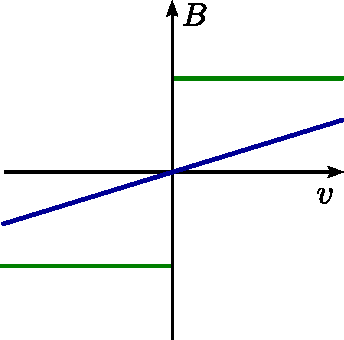
\includegraphics[width=.25\textwidth]{figures/coulombViscous1}%\vspace{-11pt}
  }
  \hspace{20pt}
  \captionbox 
  {
    coulombViscous2
    \label{fig:coulombViscous2}
  }
  {
    %\hspace{-1cm}
    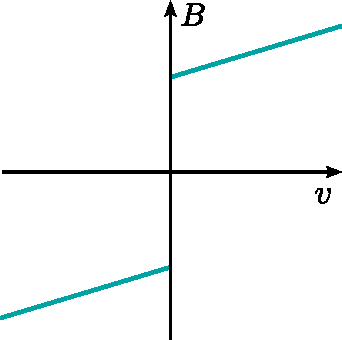
\includegraphics[width=.25\textwidth]{figures/coulombViscous2}\vspace{6pt}
  }  
\end{figure}
%
The Coulomb and viscous friction as sketched in \autoref{fig:coulombViscous1} and \ref{fig:coulombViscous2} are described by the following relations for the pendulum and cart respectively,
\begin{flalign}
  B_p(\dot{\theta}) &= b_{p,v} \dot{\theta} + \text{sgn}(\dot{\theta}) b_{p,c}        & \unit{N}  \\
  B_c(\dot{x})      &= b_{c,v} \dot{x}      + \text{sgn}(\dot{x}) b_{c,c}   \ \ \ .   & \unit{N}
  \label{eq:friction}
\end{flalign}
\begin{where}                                                                     % written out SI
  \va{ b_{p,v}   }{is the pendulum viscous friction}  {N \cdot m \cdot s}         % [kg m s^-2]
  \va{ b_{p,c}   }{is the pendulum coulomb friction}  {N \cdot m}                 % [kg s^-1]
  \va{ b_{c,v}   }{is the cart viscous friction}      {N \cdot m^{-1} \cdot s}    % [kg m^2 s^-2]
  \va{ b_{c,c}   }{is the cart coulomb friction}      {N}                         % [kg m^2 s^-1]
\end{where}

The sign-function used in \autoref{eq:friction} is undesired, as it introduces a discontinuity at zero velocity. A commonly used continuous approximation of the Coulomb friction is achieved using a tanh-function with a constant, $\text{k}_\text{tanh}$, to adjust the curve's steepness around zero.
%
\begin{figure}[H]
  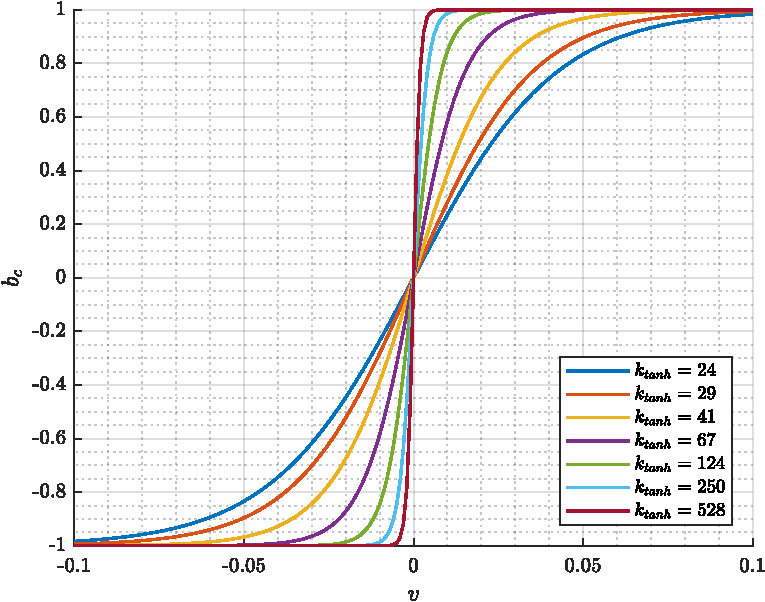
\includegraphics[width=.5\textwidth]{figures/tanhApprox}
  \caption{tanhApprox}
  \label{fig:tanhApprox}
\end{figure}

\autoref{fig:tanhApprox} shows the tanh approximation with different values of $\text{k}_\text{tanh}$. The friction parameters were estimated by a previous group who chose $\text{k}_\text{tanh} = 250$, so it makes sense to choose the same. Further, by comparing the curves in \autoref{fig:tanhApprox} the choice of $\text{k}_\text{tanh}$ seems a reasonable compromise between size of constant and steepness of the curve. The final friction model is then given by,
%
\begin{flalign}
  B_p(\dot{\theta}) &= b_{p,v} \dot{\theta} + \tanh(\text{k}_\text{tanh}\dot{\theta}) b_{p,c}        & \unit{N}  \\
  B_c(\dot{x})      &= b_{c,v} \dot{x}      + \tanh(\text{k}_\text{tanh}\dot{x}) b_{c,c}   \ \ \ .   & \unit{N}
  \label{eq:frictionTanh}
\end{flalign}

The input force so far is represented by $F$, which is directly applied in the positive $x$ direction on the cart. As seen in the beginning of this chapter in \autoref{fig:systemSetup}, this force is applied by a motor mounted with a belt on pulleys.
Because the motor control unit\fxnote{refer system description} is set up in current control mode the electrical motor dynamics are already accounted for. The controllable input is therefore the motor current, $i_a$. The torque, $\tau_m$ of the motor is modeled as directly proportional to the motor current by a torque constant, $k_\tau$, as stated in \textit{Motors} \autoref{sec:motors},
%
\begin{flalign}
  \tau_m &= k_\tau i_a       & \unit{N \cdot m}  
  \label{eq:motorTorque}
\end{flalign}

To translate this torque to the belt it is divided by the radius, $r$, of the pulley,
\begin{flalign}
  F &= \tfrac{1}{r} k_\tau i_a       & \unit{N}  
  \label{eq:motorForce}
\end{flalign}


